\section{Pengujian}
	Aplikasi yang telah dibangun dapat dikatakan berhasil jika sudah memenuhi kebutuhan fungsional dan nonfungsional yang telah didefinisikan pada tabel \ref{tabel-fungsional} dan \ref{tabel-non-fung}. Pada bab ini akan dibahas mengenai pengujian dan evaluasi pada aplikasi yang dikembangkan. Pengujian yang dilakukan terdiri dari dua pengujian yaitu pengujian fungsionalitas sistem dan pengujian statistik. Pengujian fungsionalitas mengacu pada kebutuhan fungsionalitas yang didefinisikan pada tabel \ref{tabel-fungsional}. Sedangkan pengujian statistik dilakukan untuk menguji apakah aplikasi telah memenuhi kebutuhan nonfungsional yang telah didefinisikan pada tabel \ref{tabel-non-fung}. Sebagai penutup, subbab \textit{Summary} (subbab \ref{summary-pengujian}) merangkum dan menyimpulkan hasil pengujian.

	
	\subsection{Metode Pengujian}
		
	Metode pengujian dirancang sesuai dengan kebutuhan fungsional dan nonfungsional yang telah didefinisikan. Metode-metode pengujian yang digunakan pada tugas akhir ini adalah sebagai berikut:
	
	\begin{enumerate}
	\item \textbf{Pengujian Fungsionalitas} \\
	Pengujian fungsionalitas sistem dilakukan secara mandiri dengan menyiapkan sejumlah skenario. Deskripsi proses pengujian secara lengkap akan dijelaskan pada subbab \ref{uji-fungsional}.
	
	\item \textbf{Pengujian Performa}\\
	Pengujian performa dilakukan pada setiap kasus penggunaan, dan mencatat waktu yang dibutuhkan untuk menampilkan sebuah halaman dan atau melakukan sebuah \textit{request} ke aplikasi. Deskripsi proses pengujian performa akan secara lengkap dijelaskan pada subbab \ref{uji-performa}.
	
	\item \textbf{Pengujian \textit{User Experience}} \\
	Pengujian \textit{user experience} dilakukan secara statistik, untuk menguji apakah bahwa benar aplikasi yang dibangun memberikan \textit{positive user experience} kepada penggunanya. \textit{Key performance indicator} yang digunakan didasarkan pada paper ``Development of an Instrument Measuring User Satisfaction of the Human-Computer Interface''. Deskripsi proses pengujian performa akan secara lengkap dijelaskan pada subbab \ref{uji-ux}.
	
	\item \textbf{Pengujian \textit{Maintainability}} \\
	Pengujian \textit{maintainability} dimaksudkan untuk menguji apakah benar aplikasi yang dibangun bersifat \textit{maintainable} kepada \textit{developer}. Pengujian ini dilakukan secara statistik, dengan mengacu kepada paper ``A Software Maintainability Evaluation Methodology''. Deskripsi proses pengujian secara lengkap akan dijelaskan pada subbab \ref{uji-maintainability}.
	\end{enumerate}

		
	\subsection{Pengujian Fungsionalitas}
	\label{uji-fungsional}
			
	\subsubsection{Pengujian Fungsionalitas Manajemen Autentikasi}	
		\LTXtable{\textwidth}{Chapters/Details/bab5/fungsionalitas/table/1-akun}
	
	%insert gambar here ada 3 gambar
	%deskripsi singkat
%	\documentclass{ta-its}
\usepackage{hyperref}
\usepackage{cleveref}
\usepackage{multirow}
\usepackage{graphicx}
\usepackage{array}
\usepackage{multirow}
\usepackage{tabularx}
\usepackage{tabulary}
\usepackage{etoolbox}
\usepackage{listings}
\usepackage{longtable}
\usepackage{float}
\usepackage{slantsc}
\usepackage{booktabs}% http://ctan.org/pkg/booktabs


\newcolumntype{L}[1]{>{\raggedright\let\newline\\\arraybackslash\hspace{0pt}}m{#1}}
\newcolumntype{C}[1]{>{\centering\let\newline\\\arraybackslash\hspace{0pt}}m{#1}}
\newcolumntype{R}[1]{>{\raggedleft\let\newline\\\arraybackslash\hspace{0pt}}m{#1}}

\newcommand{\mychapter}[2]{
    \setcounter{chapter}{#1}
    \setcounter{section}{0}
    \chapter*{#2}
    \addcontentsline{toc}{chapter}{#2}
}


\title{Rancang Bangun Aplikasi \textit{web} Lelang \textit{Online} \textit{(E-Auction)} Berbasis Kerangka Kerja Laravel}{E-Auction Web Application Design and Implementation based on Laravel Framework}{KI141502} 

% \author{Nama Lengkap}{NRP}
\author{Ronauli Silva Natalensis Sidabukke}{5113100142}

% \supervisorOne{Nama Pembimbing Satu}{NIP}
% \supervisorTwo{Nama Pembimbing Dua}{NIP}
\supervisorOne{Rully Soelaiman, S.Kom, M.Kom}{197002131994021001}
\supervisorTwo{Rizky Januar Akbar, S.Kom., M.Eng}{198701032014041001}

% \degree{Nama Gelar}{Bidang Studi}{Program Studi}{Jurusan}{Jurusan (English)}{Fakultas}{Fakultas Singkatan}{Fakultas (English)}
\degree{Sarjana Komputer}{Algoritma Pemrograman}{S1}{Teknik Informatika}{Informatics}{Teknologi Informasi}{FTIf}{Information Technology}

% \time{bulan}{tahun}
\time{Juni}{2017}


\begin{document}
    \maketitle
    \pagenumbering{roman}
    \legalityPaper
    \begin{abstrak}
		Industri e-commerce berkembang dengan pesat di Indonesia, seiring dengan meningkatnya jumlah pengguna internet dan menjamurnya bisnis online atau sering disebut \textit{online shop}. Salah satu jenisnya adalah lelang online, yaitu metode jual beli yang mengintegrasikan mekanisme lelang dengan Internet.
	    \newline
	    \indent Dalam interaksi antara pelaku lelang online (penjual dan pembeli) pasti terjadi kegagalan/ketidakpuasan dalam transaksi lelang online.Berangkat sebuah paper yang membahas mengenai analisa kesalahan dan strategi lewat survey terhadap pengguna aplikasi lelang online di Taiwan, penulis membangun aplikasi lelang online yang disertai dengan tambahan fitur maupun saran dari paper tersebut.
	    \newline 
	    \indent Tidak hanya berdasarkan paper rujukan, penulis juga menganalisa aplikasi \textit{e-commerce} yang umum digunakan di Indonesia baik \textit{user experience} maupun alur transaksi, dan menambahkan beberapa fitur agar lebih sesuai dengan transaksi jual-beli online yang umum di Indonesia. Dengan aplikasi ini, diharapkan kegagalan dalam transaksi online dapat diperbaiki dan membuka peluang lelang online untuk meramaikan industri \textit{e-commerce} di Indonesia.\\
\noindent \textbf{Kata-Kunci}: \textit{lelang online}, \textit{strategi }
\end{abstrak}
    \begin{abstract}
	E-commerce industry is growing rapidly in Indonesia, along with the increasing number of internet users and number of online shops is also growing. One of e-commerce type is online auction, a buy and sell method that integrates auction mechanism and the Internet.\\
	\indent In the interaction between online auction actors (buyers and sellers), inevitable failure/dissatisfaction of online auction transactions sometimes found. Started by analysing paper about online auction application typologies and strategies through an application's users survey, author want to build online auction application along with additional ideas and suggestions from the paper.  \\
	\indent Author also analyzed and considering user experience, design and transaction flow local e-commerce platforms that are commonly used in Indonesia, in purpose to make the application suits Indonesian's users better. Furthermore, author hopes that this applications can reduce/prevent the expected failures in online transactions and open up online auction opportunity to enliven the e-commerce industry in Indonesia.\\
\noindent \textbf{Keyword}: \textit{online auction}, \textit{typologies and strategies}
\end{abstract}
    \mychapter{0}{KATA PENGANTAR}
%   \begin{figure}[h]
%     \centering
%     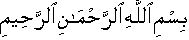
\includegraphics[width=0.5\linewidth]{images/bab0/gambarBismillah}
%   \end{figure}
	  Puji Syukur kepada Tuhan yang Maha Esa, atas berkatNya penulis dapat menyelesaikan buku berjudul \textbf{\judul}. 
	  \newline
	  \indent Selain itu, pada kesempatan ini penulis menghaturkan banyak terima kasih kepada pihak-pihak yang tanpa mereka, penulis tidak akan dapat menyelesaikan buku ini dengan baik :
  \begin{enumerate}
  	\item \textbf{\textit{Daddy Jesus}} - atas segala berkat, limpahan karunia, kesempatan dan rancangan jalanNya-lah penulis masih diberi nafas kehidupan, waktu, tenaga dan pikiran untuk menyelesaikan buku ini. \textit{Thank you, Big Daddy.}
    \item \textbf{Papa dan Mama} yang selalu menguatkan, menasehati, dan luar biasa sabar dalam mengingatkan penulis agar tidak lupa menjaga kesehatan dan tidak lupa ke gereja selama masa studi.
    \item \textbf{Yth Bapak Rully Soelaiman} yang mengajarkan penulis \textit{how to think scientifically} juga bimbingan, nasehat, saran dan memberikan penulis sisi pemikiran dan perspektif lain terhadap setiap masalah.
    \item \textbf{Yth Bapak Rizky Januar Akbar} sebagai dosen pembimbing yang memberi bimbingan, saran teknis dan administratif, diskusi dan pemecahan masalah dalam pembuatan dan penulisan buku tugas akhir.
    \item \textbf{Keluarga XL Future Leader Scholarship Camp Batch 5 \& KSE ITS} yang telah menyadarkan, memberikan semangat dan inspirasi untuk terus melanjutkan tugas akhir di saat penulis kehilangan semangat.
    \item \textbf{Keluarga Admin Lab. Pemrograman (2014 - 2017)}, yang telah memberikan penulis banyak pengalaman, pengetahuan dan cerita-cerita untuk dikenang.
    \item  \textbf{Keluarga Pengpro \textit{Furions} dan HMTC Optimasi 2016 }, yang mengajarkan penulis tentang cara berorganisasi, cara berbicara di depan publik, dan banyak lagi. 
    \item Bang Christo yang sudah jadi inspirasi dan semangat kuliah penulis sejak tahun pertama masa studi penulis sampai saat ini.  
    \item \textbf{Keluarga Alumni Budi Mulia Siantar-Surabaya angkatan 2013 }, teman setia disaat suka maupun duka. 
    \item Serta semua pihak yang tidak tertulis - yang telah turut membantu penulis dalam menyelesaikan Tugas Akhir ini.
  \end{enumerate}
  
  \indent Penulis menyadari bahwa Tugas Akhir ini masih memiliki banyak kekurangan. Oleh karena itu, penulis berharap kritik dan saran dari pembaca sekalian untuk memperbaiki buku ini ke depannya.

  \hfill Surabaya, Juli 2017 \\ \\ 


  \hfill Ronauli Silva N. Sidabukke

\cleardoublepage % Mengisi penanda halaman genap yang kosong


    \tableofcontents % Daftar isi
    \listoftables % Daftar tabel
    \listoffigures % Daftar gambar

  \mainmatter % Halaman utama, dengan judul BAB X
    \chapter{PENDAHULUAN}
  Pada bab ini akan dipaparkan mengenai garis besar Tugas Akhir yang meliputi latar belakang, tujuan, rumusan dan batasan permasalahan, metodologi pembuatan Tugas Akhir, dan sistematika penulisan.
  \section{Latar Belakang}
  	
	\indent Transaksi jual beli saat ini sudah dapat dilakukan lewat berbagai cara, antara lain menggunakan \textit{e-commerce}, atau lewat \textit{social media}, atau bisa dengan melelang di aplikasi lelang \textit{online}. Sedikit berbeda dengan teknik penjualan di lelang online, karena aplikasi ini dapat diakses oleh banyak orang, tentu saja pelelang (\textit{auctioneer}) tidak terbatas pada ruang lelang saja, tapi bisa berasal dari manapun selama mereka mengakses aplikasi tersebut.  Lelang \textit{online} ini tentu saja mendatangkan banyak manfaat, selain biaya yang lebih efisien dan hemat, dan juga tidak menguras waktu karena siapapun, kapanpun, dimanapun dapat mengajukan penawaran ataupun melelang barangnya tanpa harus pergi ke instansi tertentu dan melakukan lelang dengan cara konvensional.
    \\
    \indent Aplikasi serupa telah banyak, namun banyak aspek yang kurang dalam aplikasi tersebut, seperti informasi dari lelang tidak \textit{reliable} (misal: stok barang ternyata sudah habis), alur proses yang tidak jelas sehingga membingungkan pengguna aplikasi, informasi yang kurang jelas, dan produk yang didapatkan ternyata tidak sesuai dengan informasi pada saat produk dilelang (\textit{bad information}) \cite{ying-feng_kuo_online_2016}.
    \\
    \indent Dan dari masalah teknis aplikasi, beberapa sumber menyatakan bahwa ketidakjelasan alur proses yang kurang diperhatikan oleh para developer aplikasi lelang \textit{online} menjadi beberapa alasan yang kuat mengapa lelang online masih kurang diminati \cite{noauthor_sistem_nodate}.
    \\
	\indent Diharapkan, dengan adanya aplikasi ini, beberapa kelemahan yang masih ada pada aplikasi lelang \textit{online} saat ini dapat diperbaiki, dan juga dapat dapat membantu proses \textit{online} yang ada di Indonesia, dan juga mampu memperbaiki citra aplikasi lelang \textit{online} sehingga mampu meningkatkan minat masyarakat terhadap lelang \textit{online}.
    
  \section{Rumusan Masalah}
    Rumusan masalah yang diangkat dalam tugas akhir ini adalah sebagai berikut: 
    \begin{enumerate}
      \item Bagaimana membangun aplikasi lelang online berbasis web?
      \item Bagaimana rancangan arsitektur aplikasi dan fitur yang menganalisa kelemahan aplikasi serupa dan strategi penyelesaian sesuai dengan paper acuan \cite{ying-feng_kuo_online_2016}?
    \end{enumerate}

  \section{Batasan Masalah}
  	\label{batasan-masalah}
    Dari permasalahan yang telah diuraikan di atas, terdapat beberapa batasan masalah pada tugas akhir ini, yaitu:
    \begin{enumerate}
      \item Aplikasi berbasis web dengan bahasa pemrograman PHP.
      \item Aplikasi berbasis kerangka kerja Laravel.
      \item Basis data yang digunakan adalah PostgreSQL.
      \item Aplikasi tidak mencakup proses pembayaran.
    \end{enumerate}

  \section{Tujuan}
  \label{tujuan}
    Tujuan dari pengerjaan Tugas Akhir ini adalah: 
    \begin{enumerate}
      \item Membangun aplikasi lelang online berbasis web yang lebih kredibel sesuai dengan paper yang dijadikan acuan pada tugas akhir ini. 
    \end{enumerate}
    \chapter{LANDASAN TEORI}{}
  \section{Lelang Daring / Lelang \textit{Online}}
   Lelang adalah proses membeli dan menjual barang atau jasa dengan cara menawarkan kepada penawar, menawarkan tawaran harga lebih tinggi, dan kemudian menjual barang kepada penawar harga tertinggi. Dalam teori ekonomi, lelang mengacu pada beberapa mekanisme atau peraturan perdagangan dari pasar modal. \\
	Sementara lelang daring atau lelang melalui internet muncul seiring dengan perkembangan internet. Barang atau jasa yang diperjualbelikan dipasang di situs dan peserta lelang dapat mengikuti acara lelang secara daring. Perusahaan lelang yang berhasil menggunakan sarana internet salah satunya adalah \textit{Ebay} . Di Indonesia, lelang melalui internet (online) sudah dipelopori oleh pemerintah dengan situs lelang online yang dapat diakses melalui website resmi \href{https://www.lelangdjkn.kemenkeu.go.id}{Kemenkeu} \cite{wikipedia_lelang_2016} . 
    Berikut adalah beberapa istilah yang ada dalam lelang online :
    \begin{enumerate}
	\item BID atau \textit{Bidding}, artinya : Menawarkan
    \item BIN (\textit{Buy In Now}) artinya : Beli sesuai harga yang telah ditawarkan penjual
    \item INC (\textit{Increment}) artinya : Minimum kenaikan \textit{bid} setelah \textit{bid} sebelum nya \cite{noauthor_arti_nodate}
    \end{enumerate}
    
    \section{PostgreSQL}
    PostgreSQL adalah sebuah produk \textit{database} relasional yang termasuk dalam kategori \textit{free open source software} (\textit{FOSS}). 
	PostgreSQL terkenal karena fitur-fitur yang advanced dan pendekatan rancangan modelnya menggunakan paradigma \textit{object-oriented}, sehingga sering dikategorikan sebagai \textit{Object Relational Database Management System} (ORDBMS).
    Beberapa fitur PostgreSQL adalah sebagai berikut :
    \begin{enumerate}
    \item \textit{Inheritance}, dimana satu table dapat diturunkan model dan beberapa karakteristik dari table lainnya.
    \item \textit{Multi-Version Concurrency Control} dimana user diberi data snapshot ketika suatu perubahan dilakukan sampai commit.
    \item \textit{Rules} , dimana suatu \textit{query} DML yang dikirimkan ke server akan mengalami penulisan ulang (\textit{rewrite}). Ini terjadi sebelum diproses oleh \textit{query planner}.
    \item dan berbagai fitur lainnya \cite{noauthor_postgresql_nodate}
    \end{enumerate}
    
  \section{Redis}
    Redis adalah \textit{open source}, struktur data yang ditempatkan di memori, digunakan sebagai \textit{database}, \textit{cache} dan \textit{message broker}. Redis mendukung struktur data seperti \textit{string, sets, hash, lists} dan \textit{sorted sets}. Sama seperti cache, setiap key diisi oleh value. Tapi kelebihannya, Redis bisa digunakan untuk melakukan operasi dari value tersebut. Cara terbaik untuk memahami redis adalah membuat model aplikasi tanpa memikirkan bagaimana caranya untuk menyimpan data di dalam \textit{database} \cite{yudana_redis_2015}.

  \section{Node.js}
  Node.js adalah platform perangkat lunak pada sisi-server dan aplikasi jaringan. Ditulis dengan bahasa javascript dan bisa dijalankan pada Windows, Mac OS X dan Linux tanpa perubahan kode program. Node.js memiliki pustaka server HTTP sendiri sehingga memungkinkan untuk menjalankan webserver tanpa menggunakan program webserver seperti Apache atau Lighttpd \cite{noauthor_node.js_2014}.
  
  \section{Socket.io}
	Socket.io adalah \textit{library} Javascript untuk aplikasi web yang bersifat \textit{realtime}. Socket.io menjembatani antara komunikasi dua arah antara \textit{web} \textit{clients} dan \textit{server}. Socket.io terbagi menjadi dua bagian, yaitu \textit{client}-\textit{side} \textit{library} yang berjalan di browser client, dan \textit{server}-\textit{side} \textit{library} yang menggunakan Node.js. Kedua komponen tersebut mempunyai API yang sama. Seperti Node.js, Socket.io juga bersifat \textit{event}-\textit{driven}. Socket.IO menggunakan protokol \textit{websocket} dengan \textit{polling} sebagai opsi \textit{fallback}. Meskipun Socket.IO merupakan ‘pembungkus’ untuk soket web, namun ia memiliki banyak fitur, antara lain broadcast ke banyak soket, dan I/O yang asinkronus \cite{noauthor_socket.io_2016}.
    
    \section{Laravel}
    Laravel adalah \textit{framework} PHP yang dikembangkan pertama kali oleh Taylor Otwell. Walaupun termasuk baru, namun komunitas pengguna laravel sudah berkembang pesat dan mampu menjadi alternatif utama dari sejumlah \textit{framework} besar seperti CodeIgniter dan Yii. Laravel oleh para \textit{developer} disetarakan dengan CodeIgniter dan FuelPHP namun memiliki keunikan tersendiri dari sisi \textit{coding}. Laravel memiliki beberapa keunggulan, diantaranya :
\begin{enumerate}
\item Sintaks yang sederhana dan \textit{programmer}-\textit{fiendly}
\item Tersedia \textit{generator} yang canggih dan memudahkan, Artisan CLI
\item Fitur \textit{Schema} \textit{Builder} untuk berbagai \textit{database}
\item Fitur \textit{Migration} dan \textit{Seeding} untuk berbagai \textit{database}
\item Fitur \textit{Query} \textit{Builder} yang powerful
\item Eloquent ORM (\textit{Object} \textit{Relational} \textit{Mapping})
\item Fitur pembuatan \textit{package} dan \textit{bundle}
\item \textit{Dependency} \textit{Injection} \cite{a}
\end{enumerate}

	\section{Protokol SMTP}
    
	\section{JSON Web Token}
    
   \section{Service Worker}
   
   \section{Repository Pattern}
   
   \section{Concurrency}
   
   \section{Transaction Isolation}
   
   \section{Script Testing}
   
   \section{Laravel Dusk}
   
   


    \chapter{ANALISA DAN PERANCANGAN SISTEM}  
  \input{Chapters/Details/bab3/3a-Analisa}
  
  
%  \subsection{Perancangan Sistem}
  \input{Chapters/Details/bab3/3c-Rancangan}
  
  
    w\chapter{IMPLEMENTASI}
  Pada bab ini dibahas mengenai implementasi aplikasi sesuai dengan perancangan sistem yang telah dijelaskan sebelumnya. Bahasa pemrograman yang digunakan antara lain PHP, SQL, Javascript.
  
  \section{Lingkungan Implementasi}
  Lingkungan pembangunan dijelaskan pada subbab ini.
  \subsection{Lingkungan Pembangun Perangkat Keras}
  Perangkat keras yang digunakan dalam pembuatan tugas akhir ini adalah sebagai berikut :
  \begin{enumerate}
  \item Personal Komputer
  		\begin{enumerate}
  		\item Prosesor XX
        \item Memori YY
        \item Sistem Operasi ZZ
  		\end{enumerate}
  \item VPS
  	VPS yang digunakan dalam lingkungan pembangunan di\textit{host} oleh DigitalOcean dengan spesifikasi sebagai berikut :
  		\begin{enumerate}
  		\item Prosesor XX
        \item Memori YY
        \item Sistem Operasi ZZ
  		\end{enumerate}
  \end{enumerate}
  
  \subsection{Lingkungan Pembangun Perangkat Lunak}
  Spesifikasi perangkat lunak yang digunakan untuk membuat tugas akhir ini adalah sebagai berikut:
  \begin{enumerate}
  \item Web Browser Google Chrome
  \item PgAdmin
  \item PHPStorm sebagai IDE PHP
  \item Nano untuk \textit{shell text editor}
  \item Postman
  \item Power Designer
  \end{enumerate}
  
\section{Implementasi Antarmuka}
	
    \subsection{Antarmuka Halaman A}
    Penjelasan otorisasi terhadap antarmuka A, link yang tersedia dalam antarmuka A, dan penjelasan \textit{exception} jika terjadi masalah baik otorisasi ataupun autentikasi saat mengakses antarmuka ini.
  
      \begin{figure}[H]
        \centering
        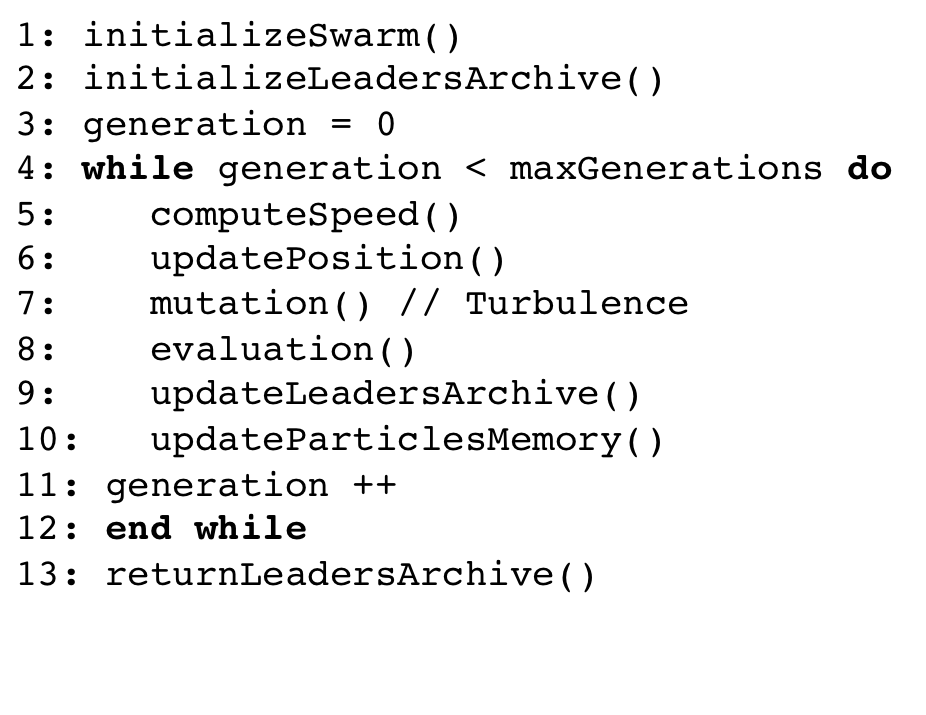
\includegraphics[width=\linewidth]{images/bab4/smpso_code.png}
        \caption{ Pseudocode Controller untuk Menampilkan Antarmuka A }
        \label{pdm}
      \end{figure}
      
    \subsection{Antarmuka Halaman B}
    Penjelasan otorisasi terhadap antarmuka B, link yang tersedia dalam antarmuka B, dan penjelasan \textit{exception} jika terjadi masalah baik otorisasi ataupun autentikasi saat mengakses antarmuka ini.
  
      \begin{figure}[H]
        \centering
        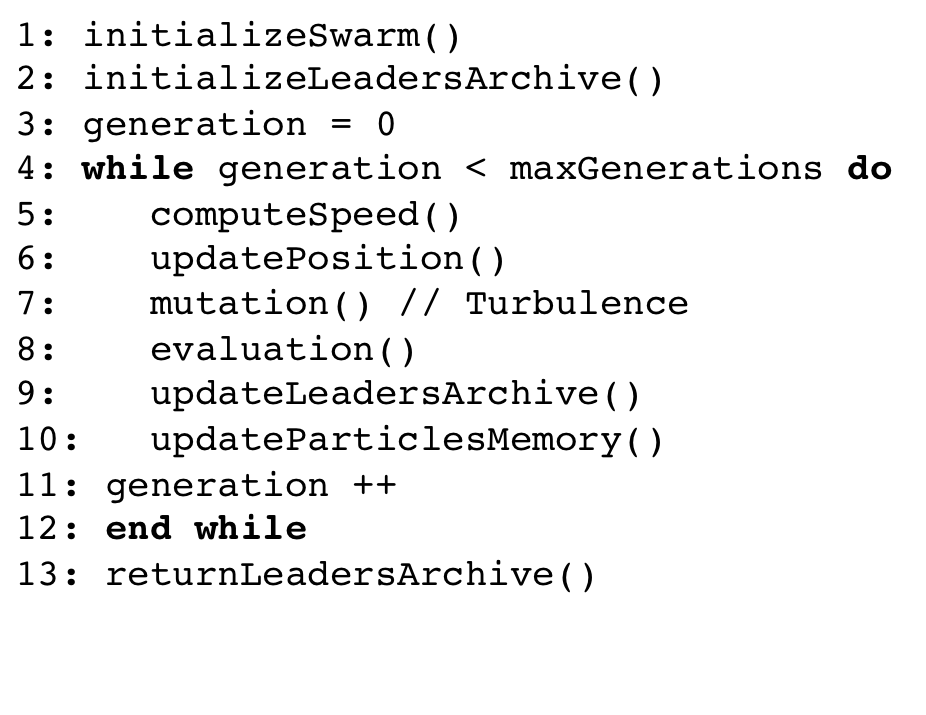
\includegraphics[width=\linewidth]{images/bab4/smpso_code.png}
        \caption{ Pseudocode Controller untuk Menampilkan Antarmuka B }
        \label{pdm}
      \end{figure}
    
    
\section{Pemasangan Proyek}
	Pembangunan dilakukan secara online, dan tersebar (tidak hanya menggunakan satu \textit{service provider} saja.
    Berikut dijelaskan langkah-langkah pembangunan proyek:
    
    \subsection{Konfigurasi Domain}
    Domain yang dipilih berasal dari Namecheap.com , dengan langkah-langkah konfigurasi sebagai berikut :
    \begin{enumerate}
    \item Langkah 1
    \item Langkah 2
    \end{enumerate}
    \subsection{Konfigurasi VPS}
    Domain yang dipilih berasal dari DigitalOcean dan Google Cloud Computing , dengan langkah-langkah konfigurasi sebagai berikut :
    \begin{enumerate}
    \item DigitalOcean
      \begin{enumerate}
      \item Langkah 1
      \item Langkah 2
      \end{enumerate}
    \item Google Cloud Computing
      \begin{enumerate}
      \item Langkah 1
      \item Langkah 2
      \end{enumerate}
    \end{enumerate}
    
    \subsection{Konfigurasi PostgreSQL}
    PostgreSQL diinstal dalam VPS, dengan langkah-langkah konfigurasi sebagai berikut :
    \begin{enumerate}
    \item Langkah 1
    \item Langkah 2
    \end{enumerate}
    
    \subsection{Konfigurasi Node.js}
    Node.js diinstall dalam VPS, dengan langkah-langkah konfigurasi sebagai berikut :
    \begin{enumerate}
    \item Langkah 1
    \item Langkah 2
    \end{enumerate}
    
    \subsection{Konfigurasi MongoDB}
    MongoDB diinstall dalam VPS, dengan langkah-langkah konfigurasi sebagai berikut :
    \begin{enumerate}
    \item Langkah 1
    \item Langkah 2
    \end{enumerate}
    
    \subsection{Konfigurasi SMTP Service}
    SMTP \textit{service} yang digunakan berasal dari sendgrid.net, dengan langkah-langkah konfigurasi sebagai berikut :
    \begin{enumerate}
    \item Langkah 1
    \item Langkah 2
    \end{enumerate}

    	\chapter{PENGUJIAN DAN EVALUASI}

	Pada bab ini akan dibahas mengenai pengujian dan evaluasi pada aplikasi. Pengujian yang dilakukan terdiri dari dua pengujian yaitu pengujian fungsionalitas sistem dan pengujian statistik. Pengujian fungsionalitas mengacu pada daftar fungsionalitas pada bab III (Desain dan Perancangan) Sedangkan pengujian statistik dilakukan untuk membuktikan bahwa aplikasi benar telah mencapai tujuan yang dipaparkan pada Bab II poin 2.
    
      
    \input{Chapters/Details/bab5/5a-Pengujian}
    
    \input{Chapters/Details/bab5/5b-Evaluasi}
    

    %\section{Struktur Dokumen \LaTeX{}}
Dokumen \LaTeX{} terdiri dari struktur yang dibuat berdasarkan struktur dokumen sehari-hari. Sebagai penulis dokumen, Anda wajib menggunakan struktur ini sehingga \LaTeX{} dapat melakukan hal lain yang membantu Anda dalam mengorganisir dokumen seperti misalnya pembuatan Daftar Isi. Berikut adalah struktur dokumen yang ada di \LaTeX{} diurutkan berdasarkan hirarkinya.

\begin{ltabulary}{|L|L|} % L = Rata kiri untuk setiap kolom, | = garis batas vertikal.

% Kepala tabel, berulang di setiap halaman
\caption{Struktur hirarki dokumen \LaTeX{}} \label{tabelStrukturDokumen} \\
\hline
\textbf{Nama} & \textbf{Peruntukkan} \\ \hline

\endhead
\endfoot
\endlastfoot

% Isi Tabel
\textbf{\textbackslash{}part\{Judul Bagian\}} & \texttt{book} \\ \hline
\textbf{\textbackslash{}chapter\{Judul Bab\}} & \texttt{book} dan \texttt{report} \\ \hline
\textbf{\textbackslash{}section\{Judul Subbab\}} & semua kecuali \texttt{letter} \\ \hline
\textbf{\textbackslash{}subsection\{Judul Subsubbab\}} & semua kecuali \texttt{letter} \\ \hline
\textbf{\textbackslash{}subsubsection\{Judul Subsubsubbab\}} & semua kecuali \texttt{letter} \\ \hline
\textbf{\textbackslash{}paragraph\{Judul Paragraf\}} & semua\\ \hline

\end{ltabulary}

\subsection{Pengujian Performa}
      Pengujian 
      \subsubsection{Pengujian Kecepatan Fitur A}
      Pengujian fitur ini dilakukan pada lingkungan uji \ref{env_uji1}, dan untuk lebih lengkapnya dapat dilihat pada tabel \ref{uji1}
      \begin{table}[]
      \centering
      \caption{Pengujian Fitur B}
      \label{uji2}
      \begin{tabular}{llll}
      \multicolumn{1}{c}{\textbf{ID}} & \multicolumn{3}{c}{\textbf{TA-UJI.Proses}}        \\
      Referensi Proses Penggunaan     & \multicolumn{3}{l}{}                              \\
      Nama                            & \multicolumn{3}{l}{}                              \\
      Tujuan Pengujian                & \multicolumn{3}{l}{\multirow{2}{*}{}}             \\
      \textbf{Skenario Pengujian}     & \multicolumn{3}{l}{}                              \\
      Langkah Pengujian               & \multicolumn{3}{l}{}                              \\
      Kecepatan Buka Halaman          & Halaman       & \multicolumn{2}{l}{Google Chrome} \\
                                      & A             & 18 KB           & 0.987s         
      \end{tabular}
      \end{table}
      
    \chapter{PENUTUP}
  Bab ini membahas kesimpulan yang dapat diambil dari tujuan pembuatan sistem dan hubungannya dengan hasil uji coba dan evaluasi yang telah dilakukan. Selain itu, terdapat beberapa saran yang bisa dijadikan acuan untuk melakukan pengembangan dan penelitian lebih lanjut.
  \section{Kesimpulan}
  Dari proses perancangan, implementasi dan pengujian terhadap sistem, dapat diambil beberapa kesimpulan berikut:
  \begin{enumerate}
    \item Kualitas perancangan dan desain sistem dan fleksibilitas sistem sangat penting dalam rancang bangun aplikasi jual-beli online, karena sifat perubahan yang sangat cepat.
    \item \textit{User Experience} adalah faktor yang sangat penting dalam kesuksesan platform jual-beli online
    \item Selain \textit{user experience}, \textit{maintainability} juga sangat penting karena yang menjaga dan memperbarui perangkat lunak jika ada perubahan adalah \textit{developer} sendiri. Jika sebuah sistem \textit{maintainability}nya buruk, maka sistem tersebut juga tidak fleksibel terhadap perubahan karena \textit{developer} juga pasti pusing untuk menambahkan fitur yang 
  \end{enumerate}
  
  \section{Saran}
  Berikut beberapa saran yang diberikan untuk pengembangan lebih lanjut:
  \begin{enumerate}
    \item Mengikutsertakan pihak yang \textit{capable}/kredibel dan ahli di bidang hukum dan \textit{bussiness process} untuk menetapkan alur, memperbaiki alur dan membuat alur monitoring untuk proses lelang yang lebih aman, kredibel.
    \item Mempelajari platform lelang \textit{online} di luar negeri yang sudah sukses, yakni mempelajari ide-ide, alur aktivitas dan penggunaan kaidah \textit{user experience} dan \textit{usability} dalam website tersebut dan dampaknya terhadap \textit{revenue}.
  \end{enumerate}
  

    \appendix % Halaman lampiran, dengan judul LAMPIRAN X
  \backmatter % Lampiran tanpa judul LAMPIRAN X, untuk BIODATA PENULIS
\end{document}
		
	\subsubsection{Pengujian Fungsionalitas Manajemen Penawaran}
		\LTXtable{\textwidth}{Chapters/Details/bab5/fungsionalitas/table/2-penawaran}
	
	%insert gambar here ada 3 gambar
	%deskripsi singkat
		
	\subsubsection{Pengujian Fungsionalitas Manajemen Barang Lelang}
		\LTXtable{\textwidth}{Chapters\Details\bab5\fungsionalitas\table\3-barang}
	
	%insert gambar here ada 3 gambar
	%deskripsi singkat
			
	\subsubsection{Pengujian Fungsionalitas Manajemen Interaksi Antarpengguna}
			\LTXtable{\textwidth}{Chapters/Details/bab5/fungsionalitas/table/4-interaksi}
		
		%insert gambar here ada 3 gambar
		%deskripsi singkat


	
	\subsubsection{Pengujian Fungsionalitas Manajemen Laporan}
			\LTXtable{\textwidth}{Chapters/Details/bab5/fungsionalitas/table/5-laporan}
		
		%insert gambar here ada 3 gambar
		%deskripsi singkat


	
	\subsubsection{Pengujian Fungsionalitas Manajemen Kupon}
			\LTXtable{\textwidth}{Chapters/Details/bab5/fungsionalitas/table/6-kupon}
		
		%insert gambar here ada 3 gambar
		%deskripsi singkat


	
			

	
	
	\subsection{Pengujian Performa}
	\label{uji-performa}
	
	\subsubsection{Proses Pengujian}
	\input{Chapters\Details\bab5\fungsionalitas\process}
	
	\subsubsection{Hasil Pengujian}
	Hasil rekapitulasi kuisioner \textit{user experience} dapat dilihat pada Tabel \ref{user-test-recap}.
\LTXtable{\textwidth}{table/05/pengguna/recap_all}
	
	\subsection{User Experience Assesment}
	\label{[uji-ux}
		
	\subsubsection{Proses Pengujian}
	Pengujian dilakukan dengan menggunakan kriteria yang mengacu kepada paper \textbf{Development of an Instrument Measuring User Satisfaction of the Human-Computer Interface}\cite{chin_development_1998}, yaitu sebagai berikut:
\begin{enumerate}
	\item Desain \& Impresi Web
	\item Kejelasan \& Konsistensi Sistem
	\item Kemudahan Penggunaan
	\item Kejelasan status proses
	\item \textit{Error message} yang jelas
	\item Kecepatan
	\item \textit{Rating} Keseluruhan
	\item Tingkat rekomendasi pada teman
\end{enumerate}
\ \indent Pengujian ini dilakukan pada tanggal 8 Juli 2017 di Kebun Bibit Wonorejo, dengan secara sembarang memilih responden yang sedang ada di kebun tersebut. Kemudian, responden diminta untuk menggunakan aplikasi yang sudah ada sebelumnya (balelang.com) dan aplikasi tugas akhir ini selama beberapa menit, dan setelah dirasa cukup, lalu responden mengisi kuisioner yang telah diberikan.
	
	\subsubsection{Hasil Pengujian}
	Hasil rekapitulasi kuisioner \textit{user experience} dapat dilihat pada Tabel \ref{user-test-recap}.
\LTXtable{\textwidth}{table/05/pengguna/recap_all}
	
	\subsection{Maintainability Assesment}
	\label{uji-maintainability}
		
	\subsubsection{Proses Pengujian}
	Pengujian dilakukan dengan menggunakan kriteria yang mengacu kepada paper \textbf{A Software Maintainability Evaluation Methodology}\cite{peercy_software_nodate}. Paper ini menyebutkan bahwa ada 2 kriteria dasar penilaian \textit{maintainability} dengan \textit{weight} berbeda, yaitu dokumentasi (\textit{weight: 40\%}) dan \textit{source code}(\textit{weight: 60\%}). Menurut paper tersebut, terdapat 5 faktor utama \textit{maintainability}, yaitu sebagai berikut:
\begin{enumerate}
	\item \textit{modularity};
	\item \textit{descriptiveness};
	\item \textit{consistency};
	\item \textit{simplicity}; dan
	\item \textit{trackability}
\end{enumerate}

\ \indent Pengujian ini dilakukan dengan cara menyebar \textit{form online} via Google Forms. Responden yang disasar adalah responden dengan latar belakang \textit{software engineer} dengan tujuan agar responden dapat membandingkan pengalaman responden tersebut dengan kualitas \textit{maintainability} tugas akhir ini.
	
	\subsubsection{Hasil Pengujian}
	Hasil rekapitulasi kuisioner \textit{user experience} dapat dilihat pada Tabel \ref{user-test-recap}.
\LTXtable{\textwidth}{table/05/pengguna/recap_all}
	
	\subsection{\textit{Summary}}
	\label{summary-pengujian}
		
	\subsubsection{Proses Pengujian}
	Pengujian dilakukan dengan menggunakan kriteria yang mengacu kepada paper \textbf{Development of an Instrument Measuring User Satisfaction of the Human-Computer Interface}\cite{chin_development_1998}, yaitu sebagai berikut:
\begin{enumerate}
	\item Desain \& Impresi Web
	\item Kejelasan \& Konsistensi Sistem
	\item Kemudahan Penggunaan
	\item Kejelasan status proses
	\item \textit{Error message} yang jelas
	\item Kecepatan
	\item \textit{Rating} Keseluruhan
	\item Tingkat rekomendasi pada teman
\end{enumerate}
\ \indent Pengujian ini dilakukan pada tanggal 8 Juli 2017 di Kebun Bibit Wonorejo, dengan secara sembarang memilih responden yang sedang ada di kebun tersebut. Kemudian, responden diminta untuk menggunakan aplikasi yang sudah ada sebelumnya (balelang.com) dan aplikasi tugas akhir ini selama beberapa menit, dan setelah dirasa cukup, lalu responden mengisi kuisioner yang telah diberikan.
	
	\subsubsection{Hasil Pengujian}
	Hasil rekapitulasi kuisioner \textit{user experience} dapat dilihat pada Tabel \ref{user-test-recap}.
\LTXtable{\textwidth}{table/05/pengguna/recap_all}
	
		
		
